\chapter{Results}
Both models show a strong ability to predict solar irradiance one day into the future.
The full model, using weather forecast data from the surrounding area, shows both a lower Mean Absolute Percentage Error (MAPE), at 13.21\% vs. 15.98\%, as well as better tracking in challenging conditions and a better ability to recognize uncertain conditions, generally reporting lower confidence when its predictions are wrong. Both models can be trained to achieve slightly lower MAPE, but that comes at the cost of a higher tendency to underfit variance and higher false confidence.
We show irradiance plots for select days representative of the models' performance in various conditions. These plots show the measured irradiance for the day, the models' predicted irradiance values, along with a 90\% confidence interval, detailed in Section~\ref{sec:loss_function}. The plots also show the forecast downward shortwave irradiance, the largest factor in measured irradiance, from the model input. Additionally, the graphs contain the average MAPE for the day and the sum of prediction and observation values. The sum values act as a gauge for the total irradiance for the day.


\section{Full model}
The full model, utilizing irradiance data from surrounding areas achieves an average MAPE of 13.21\% on the test dataset. The maximum daily average MAPE is 138.87\% and the minimum is 2.50\%. Figure~\ref{fig:days_full} shows the average MAPE the full model achieves for the test dataset on a day-by-day basis.
\begin{figure}[ht!]
    \centering
    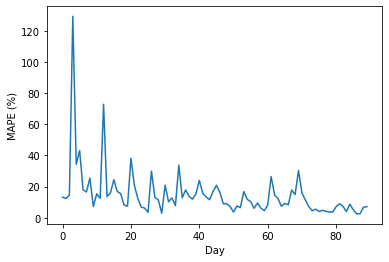
\includegraphics[scale=1]{imgs/graphs/full/days_full.png}
    \caption{The recorded Mean Absolute Percentage Error (MAPE) for each day in the test dataset for the full model. 
    \label{fig:days_full}}
\end{figure}




\subsection{Low variance days}
In the test dataset, there are some clear days, where the sun was mostly or entirely unobstructed. The model predicts most of these days with very low error, in the range of 2-5\%. The 90\% confidence interval stays within $\pm100 W/m^2$ for the whole day and the true prediction is almost spot-on, as can be seen in Figure~\ref{fig:full_low_best}.
\begin{figure}[ht!]
    \centering
    \subfloat[]{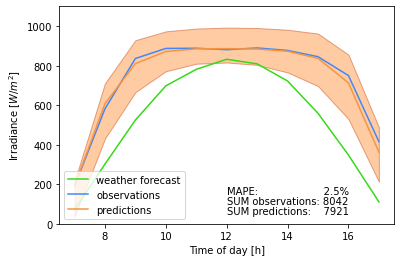
\includegraphics[scale=0.5]{imgs/graphs/full/low/best_3.png}}\qquad
    \subfloat[]{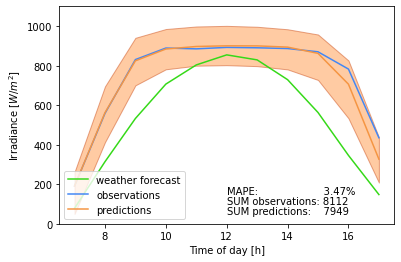
\includegraphics[scale=0.5]{imgs/graphs/full/low/best_2.png}}\qquad
    \caption{Examples of clear days where the model performs very well.
    \label{fig:full_low_best}}
\end{figure}


The model does not manage near-perfect predictions on all of these clear days, and makes a few under-predictions, as can be seen in Figure~\ref{fig:full_low_worst}.
These predictions still predict steady sunshine and are within the 90\% confidence interval, which is slightly larger than for the other clear day predictions. These predictions have a higher MAPE of 10-13\%.



\subsection{Medium variance days}
On days with some variance in the irradiance measured, the model is generally able to predict the irradiance with relatively good accuracy.
The model tends to give a smoother prediction than the measured value, averaging through the peaks and valleys of the measured values and most of the time the observed value is within the 90\% confidence interval. 

Figure~\ref{fig:full_med_best} shows examples of good predictions with high confidence, though the confidence is generally lower the farther the irradiance is from the value of a clear day.

\afterpage{%
\begin{figure}
    \centering
    \subfloat[]{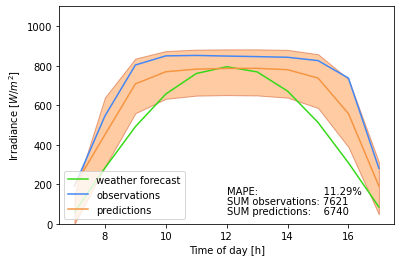
\includegraphics[scale=0.5]{imgs/graphs/full/low/worst_1.png}}\qquad
    \subfloat[]{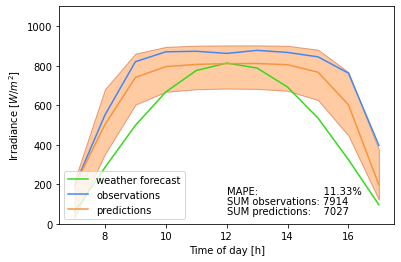
\includegraphics[scale=0.5]{imgs/graphs/full/low/worst_2.png}}\qquad
    \caption{Examples of clear days where the model does not perform well.
    \label{fig:full_low_worst}}
\end{figure}

\begin{figure}
    \centering
    \subfloat[]{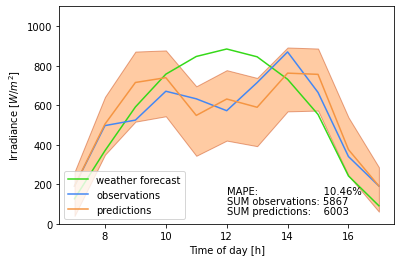
\includegraphics[scale=0.5]{imgs/graphs/full/medium/med_g_1.png}}\qquad
    \subfloat[]{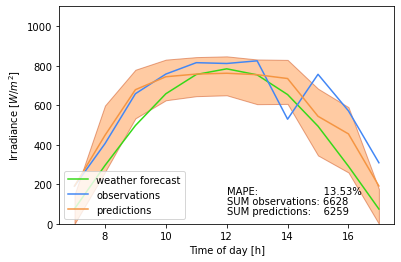
\includegraphics[scale=0.5]{imgs/graphs/full/medium/med_g_2.png}}\qquad
    \subfloat[]{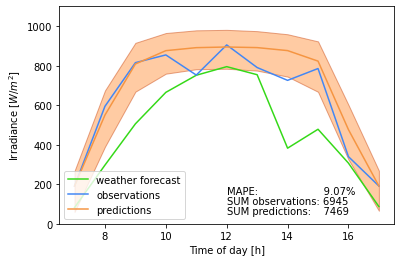
\includegraphics[scale=0.5]{imgs/graphs/full/medium/med_g_3.png}}\qquad
    \subfloat[]{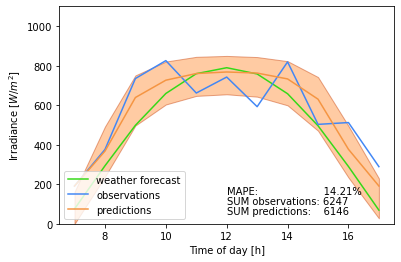
\includegraphics[scale=0.5]{imgs/graphs/full/medium/med_g_4.png}}\qquad
    \caption{Examples of days with some drops in irradiance, where the model performs very well.
    \label{fig:full_med_best}}
\end{figure}
\clearpage
}

In Figure~\ref{fig:full_med_med} we see examples of days where the model achieves higher error, MAPE in the range 19-35\%, but with generally larger 90\% confidence intervals so the model still keeps the measured values close to or within them.

\afterpage{%
\begin{figure}
    \centering
    \subfloat[]{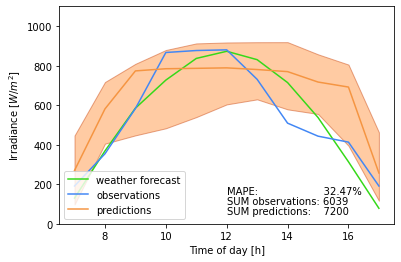
\includegraphics[scale=0.5]{imgs/graphs/full/medium/med_m_1.png}}\qquad
    \subfloat[]{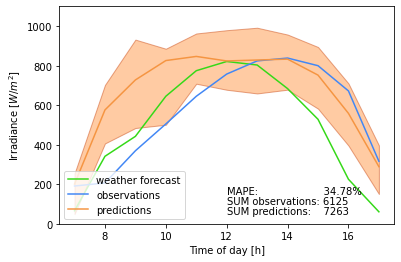
\includegraphics[scale=0.5]{imgs/graphs/full/medium/med_m_2.png}}\qquad
    \subfloat[]{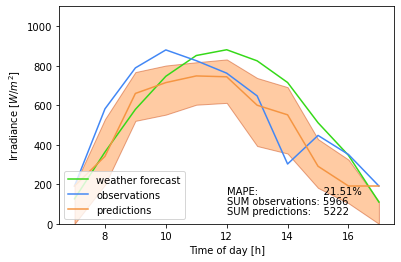
\includegraphics[scale=0.5]{imgs/graphs/full/medium/med_m_3.png}}\qquad
    \subfloat[]{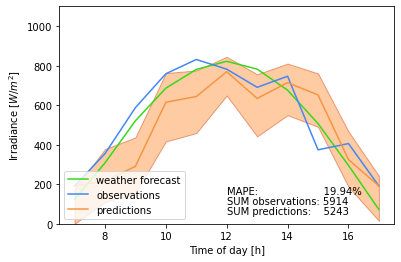
\includegraphics[scale=0.5]{imgs/graphs/full/medium/med_m_4.png}}\qquad
    \subfloat[]{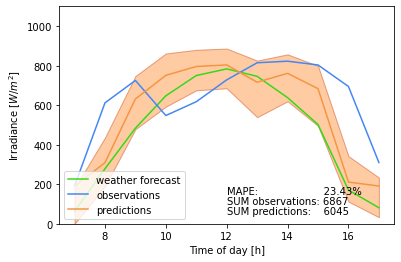
\includegraphics[scale=0.5]{imgs/graphs/full/medium/med_m_5.png}}\qquad
    \caption{Examples of days with some drops in irradiance, where the model performs somewhat well.
    \label{fig:full_med_med}}
\end{figure}
\clearpage
}

For a few medium variance days, the model does not track well. Figures~\ref{fig:full_med_bad_a} and \ref{fig:full_med_bad_d} show where the model predicts a constant lower irradiance when half the day had high irradiance and the other half low. Figures~\ref{fig:full_med_bad_b} and \ref{fig:full_med_bad_c} show the model predicting a mostly or fully sunny day when it was not. In all of these cases, the observed irradiance is far outside the 90\% confidence interval.

\afterpage{%
\begin{figure}
    \centering
    \subfloat[]{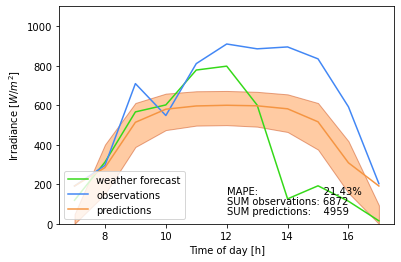
\includegraphics[scale=0.5]{imgs/graphs/full/medium/med_b_1.png}\label{fig:full_med_bad_a}}\qquad
    \subfloat[]{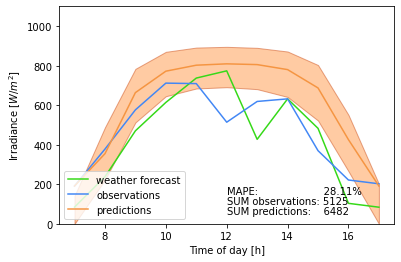
\includegraphics[scale=0.5]{imgs/graphs/full/medium/med_b_2.png}\label{fig:full_med_bad_b}}\qquad
    \subfloat[]{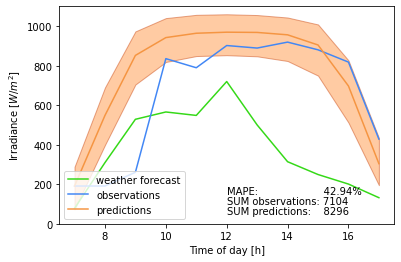
\includegraphics[scale=0.5]{imgs/graphs/full/medium/med_b_3.png}\label{fig:full_med_bad_c}}\qquad
    \subfloat[]{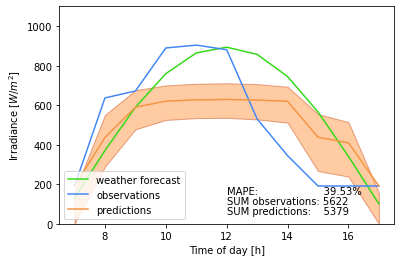
\includegraphics[scale=0.5]{imgs/graphs/full/medium/med_b_4.png}\label{fig:full_med_bad_d}}\qquad
    \caption{Examples of days with some drops in irradiance, where the model performs badly.
    \label{fig:full_med_bad}}
\end{figure}
\clearpage
}

\clearpage
\subsection{High variance days}
A few days in the dataset had very low irradiance for part of, or the whole day, or large fluctuations in irradiance. These situations are the most difficult for the model to predict. Figures~\ref{fig:full_high_a}, \ref{fig:full_high_b} and \ref{fig:full_high_c} show the model somewhat following the observations, but with a high MAPE of 38-80\% because of offsets in time and/or magnitude. The observed value is often outside the 90\% confidence interval of the predictions. For Figures~\ref{fig:full_high_a}, \ref{fig:full_high_b} the sum of predicted values is close to the sum of observed values, indicating relatively high accuracy for the days taken as a whole. Figure~\ref{fig:full_high_d} shows an outlier with an extremely high MAPE of 139\%, where the model predicts an almost clear day, with high confidence, on a day that received very little irradiance.
\begin{figure}[ht!]
    \centering
    \subfloat[]{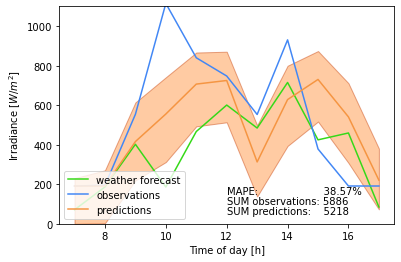
\includegraphics[scale=0.5]{imgs/graphs/full/high/high_1.png}\label{fig:full_high_a}}\qquad
    \subfloat[]{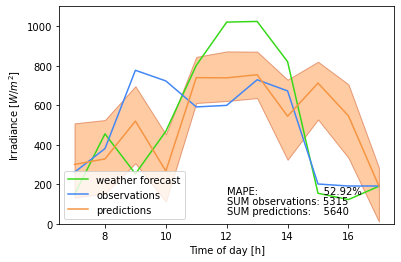
\includegraphics[scale=0.5]{imgs/graphs/full/high/high_2.png}\label{fig:full_high_b}}\qquad
    \subfloat[]{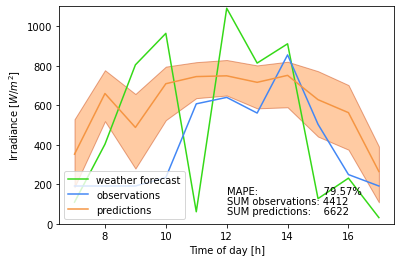
\includegraphics[scale=0.5]{imgs/graphs/full/high/high_3.png}\label{fig:full_high_c}}\qquad
    \subfloat[]{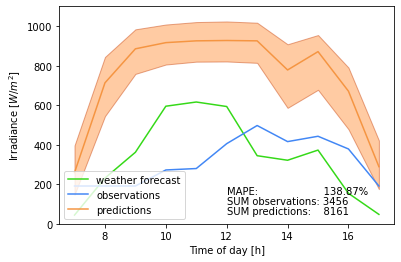
\includegraphics[scale=0.5]{imgs/graphs/full/high/high_4.png}\label{fig:full_high_d}}\qquad
    \caption{Examples of days with large drops in irradiance or low irradiance throughout.
    \label{fig:full_high}}
\end{figure}




\clearpage
\section{Less forecast data}
To confirm that the full model utilizes the input data for the surrounding area, we also trained the model on only the irradiance forecast for the cell the power station is located in.
The limited model achieves an average MAPE of 15.98\% on the test dataset. The maximum daily average MAPE is 122.87\% and the minimum is 3.47\%. Figure~\ref{fig:days_less} shows the average MAPE the limited model achieved for the test dataset on a day-by-day basis.
\begin{figure}[ht!]
    \centering
    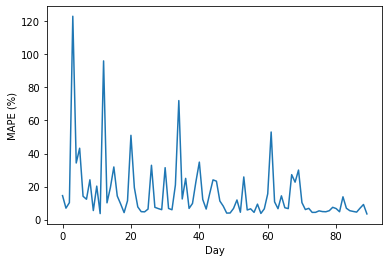
\includegraphics[scale=1]{imgs/graphs/less/days_single.png}
    \caption{The recorded Mean Absolute Percentage Error for each day in the test dataset of the limited model. 
    \label{fig:days_less}}
\end{figure}

\newpage
\subsection{Low variance days}
The model predicts most clear days with relatively high accuracy, but even on the best days, it deviates quite a bit from the observed values, as shown in Figure~\ref{fig:less_low_a}. The model sometimes under-predicts on clear days. In Figure~\ref{fig:less_low_b} we can see an example of a day where, even though the 90\% confidence area is large, the observed irradiance is outside it.
\begin{figure}[ht!]
    \centering
    \subfloat[]{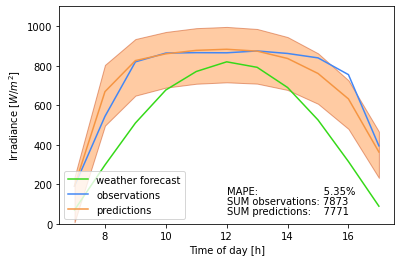
\includegraphics[scale=0.5]{imgs/graphs/less/low/low_g_1.png}\label{fig:less_low_a}}\qquad
    \subfloat[]{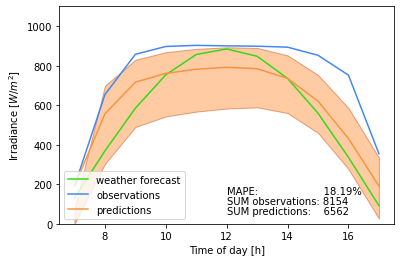
\includegraphics[scale=0.5]{imgs/graphs/less/low/low_b_1.png}\label{fig:less_low_b}}\qquad
    \caption{Examples of model performance on clear days.
    \label{fig:less_low}}
\end{figure}

\subsection{Medium variance days}
The model shows less accuracy when the irradiance is not steady. Predictions for most days have the smooth profile of an optimal day but are scaled to fit closer to the lower total irradiance for the day. The model is inconsistent in how well it tracks the observed irradiance and the confidence it does that with. Sometimes, as shown in Figure~\ref{fig:less_med_a} the model tracks relatively well, with the observations mostly within the rather tight 90\% confidence interval of roughly $+50/-150 W/m^2$. In Figure~\ref{fig:less_med_b} we see an example where the model is wrong with very high confidence for the first half of the day. Figure~\ref{fig:less_med_c} shows the opposite, the model predicts low irradiance for the whole day with a very large 90\% confidence interval of roughly $\pm200 W/m^2$.

\afterpage{%
\vspace{5cm}
\begin{figure}
    \centering
    \makebox[\textwidth][c]{\subfloat[]{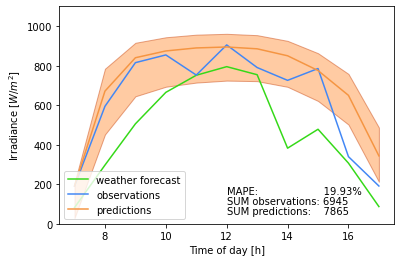
\includegraphics[scale=0.5]{imgs/graphs/less/medium/med_g_1.png}\label{fig:less_med_a}}\qquad}
    \makebox[\textwidth][c]{\subfloat[]{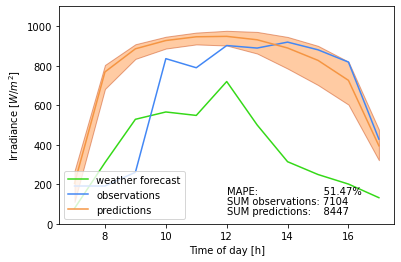
\includegraphics[scale=0.5]{imgs/graphs/less/medium/med_m_2.png}\label{fig:less_med_b}}\qquad}
    \makebox[\textwidth][c]{\subfloat[]{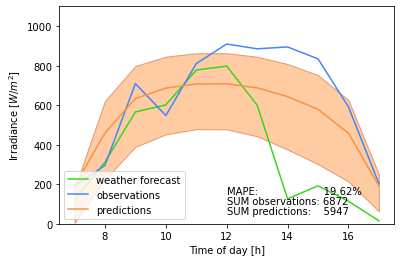
\includegraphics[scale=0.5]{imgs/graphs/less/medium/med_m_1.png}\label{fig:less_med_c}}\qquad
    }
    \caption{Examples of days with some drops in irradiance.
    \label{fig:less_med}}
\end{figure}
\clearpage
}

\clearpage
\subsection{High variance days}
For the few days in the dataset that had very low irradiance for part of, or the whole day, or large fluctuations in irradiance, the model displays a high error, MAPE in the range 53-123\% with varying confidence. Figures~\ref{fig:less_high_a} and \ref{fig:less_high_b} show large over-predictions with high confidence, and Figures~\ref{fig:less_high_c} and \ref{fig:less_high_d} show days where the 90\% confidence interval covers the top 60\% of the graph, yet it does not cover the observations.
\begin{figure}[ht!]
    \centering
    \subfloat[]{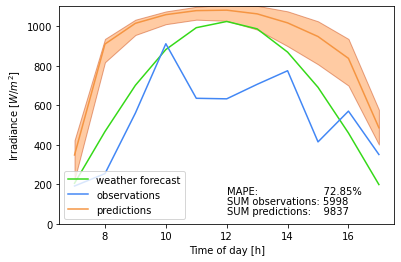
\includegraphics[scale=0.5]{imgs/graphs/less/high/high_1.png}\label{fig:less_high_a}}\qquad
    \subfloat[]{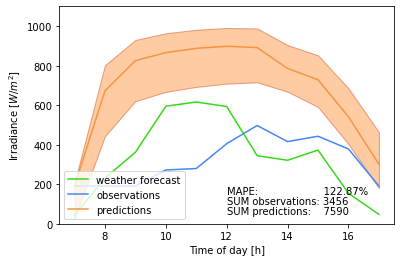
\includegraphics[scale=0.5]{imgs/graphs/less/high/high_2.png}\label{fig:less_high_b}}\qquad
    \subfloat[]{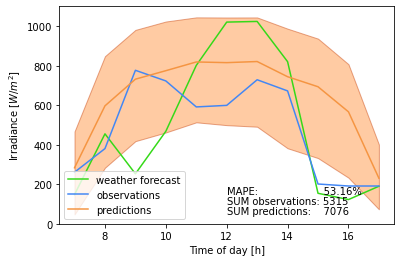
\includegraphics[scale=0.5]{imgs/graphs/less/high/high_3.png}\label{fig:less_high_c}}\qquad
    \subfloat[]{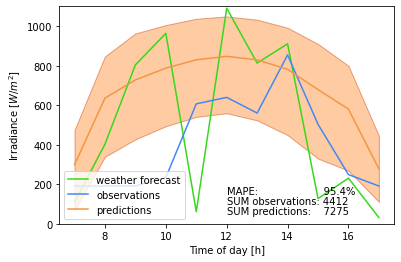
\includegraphics[scale=0.5]{imgs/graphs/less/high/high_4.png}\label{fig:less_high_d}}\qquad
    \caption{Examples of days with large drops in irradiance or low irradiance throughout.
    \label{fig:less_high}}
\end{figure}